% THIS IS SIGPROC-SP.TEX - VERSION 3.1
% WORKS WITH V3.2SP OF ACM_PROC_ARTICLE-SP.CLS
% APRIL 2009
%
% It is an example file showing how to use the 'acm_proc_article-sp.cls' V3.2SP
% LaTeX2e document class file for Conference Proceedings submissions.
% ----------------------------------------------------------------------------------------------------------------
% This .tex file (and associated .cls V3.2SP) *DOES NOT* produce:
%       1) The Permission Statement
%       2) The Conference (location) Info information
%       3) The Copyright Line with ACM data
%       4) Page numbering
% ---------------------------------------------------------------------------------------------------------------
% It is an example which *does* use the .bib file (from which the .bbl file
% is produced).
% REMEMBER HOWEVER: After having produced the .bbl file,
% and prior to final submission,
% you need to 'insert'  your .bbl file into your source .tex file so as to provide
% ONE 'self-contained' source file.
%
% Questions regarding SIGS should be sent to
% Adrienne Griscti ---> griscti@acm.org
%
% Questions/suggestions regarding the guidelines, .tex and .cls files, etc. to
% Gerald Murray ---> murray@hq.acm.org
%
% For tracking purposes - this is V3.1SP - APRIL 2009

\documentclass{acm_proc_article-sp}
\setlength{\parindent}{2em}

\begin{document}

\title{Anonymity Network: Cloud-based Onion Routing}

\numberofauthors{5} 

\author{
% 1st. author
\alignauthor
Fabian Gr�nbichler
% 2nd. author
\alignauthor
Klaus Krapfenbauer
% 3rd. author
\alignauthor
Thomas Hackl
\and  % use '\and' if you need 'another row' of author names
% 4th. author
\alignauthor 
Stefan Gamerith
% 5th. author
\alignauthor 
Milan Dzenovljanovic
}

\maketitle
\begin{abstract}
\textit{An anonymity network should enable users to access the public Internet
	while at the same time hiding their real identity (e.g., IP address) from
	prying eyes. The main focus of this paper is a class of anonymity networks
	based on Onion Routing. Connections routed through such a network are 
	strongly resistant to traffic analysis and are not limited to one specific
	protocol (e.g., HTTP(S)). In an Onion network, messages are encrypted and 
	transmitted over a set of Onion Routers. Every Onion Router removes one
	layer of encryption (like the skins of an onion),  reads the routing 
	instructions contained within and sends the rest of the content to the next
	router. This process is repeated for all nodes along a so called chain,
	where every router is only aware of the existence of the previous and next 
	node. Only the first node knows the true location (or identity) of the user,
	and only the last node knows the actual plain-text data. Today's most used 
	Onion Routing network is Tor. Because of the ever-increasing number of
	users, the Tor network often suffers from poor performance. Therefore as 
	well as for other benefits of cloud computing (broad network access, 
	resource pooling, rapid elasticity, ensured services), moving Onion Routing
	services into the ``cloud'' seems like a logical step.
This paper describes anonymous connections and their implementation using 
Cloud-based Onion Routing.
}
\end{abstract}

\terms{Security, Privacy}

\keywords{Anonymity networks, Onion Routing, Cloud computing} 

\section{Introduction}
Anonymity networks enable users to communicate over the public Internet while 
hiding their identity from one another. Nevertheless, is Internet communication 
private? One of the greatest concerns today is preventing outsiders from
listening in on electronic conversations. But \textit{traffic analysis} can also
leak some sensitive information because encrypted messages can be tracked, revealing 
who is communicating with whom. \cite{cite1}

One of today's most scrutinized as well as most popular tool for accessing the
Internet anonymously is Tor. By routing the traffic through a sequence of nodes, 
Tor allows the traffic to appear to the target as if it were originating from 
the last node, instead of from the user directly. The main disadvantage of Tor 
is that its relays are hosted by volunteers all over the world. This volunteers
mainly use private, consumer-grade ISP connections which often have limited 
bandwidth capacity, therefore Tor users often face performance issues. \cite{cite2}

Moving Onion Routing services to the ``cloud'' could bring the advantage of
being able to quickly rotate between a lot of different IP addresses as well as
adding a large number of high-quality, high-bandwidth nodes to the network. 
The biggest advantage of most cloud infrastructures lays in their ``elasticity''.
By spawning or terminating virtual machine instances in the cloud one can easily, 
quickly and automatically add or remove nodes/routers to or from an anonymity
network. \cite{cite2}

The main goal of \textit{traffic analysis} is to discover participants of 
communication, whether the participants are exchanging mails or a user is just
browsing the Web. Bearing this in mind, \textit{anonymity networks} are 
developed to mislead the observers by making it difficult to derive such 
information, which is usually stored into the packet headers or in the encrypted
payload, from the connection.

Thus, any information that carries identifying data must be sent through the 
\textit{anonymous  network}. Onion Routing is one implementation of such an
\textit{anonymous network} that stands out with comparably low latency and low
overhead. Fundamentally, Tor's protocol is an extension of Onion Routing and 
provides two-way, real-time, connection-based communication that does not 
require the target to participate in the \textit{anonymity} protocol.
All aforementioned features together make anonymising communication on the Web
easier. \cite{cite1} \cite{cite2}

\section{Onion Routing}
\subsection{Overview}

In Onion Routing, user connects to a target over a sequence of machines called
\textit{Onion Routers}, rather than connecting directly to a target.
This way the \textit{originator} can remain anonymous to an \textit{observer}. 
It is possible for the \textit{originator} to remain anonymous to the target, if
all informations that identifies the \textit{originator} has been removed from 
the plain-text data stream before it is sent over the \textit{Onion Routing network}.

\subsection{Data transfer}
In the \textit{Onion Routing network} routers communicate using TCP connections
(it could be implemented on top of other protocols as well). The set of the 
\textit{Onion Routers} in a route is defined at the very setup of the connection,
when the \textit{originator } creates an \textit{Onion}, and each router knows
only the previous and next routers along the route. An \textit{onion} is a 
layered data structure that encapsulates cryptographic information such as the 
keys or key exchange data as well as the cryptographic algorithms used during
the data transfer. Along the route each \textit{Onion Router} uses its public 
key do decrypt the entire \textit{Onion}. This way the identity of the next 
router along the route as well as the embedded \textit{Onion} is exposed. The
\textit{Onion Router} sends the \textit{Onion} to the next router, after the 
connection is established, data can be sent in both directions. Using the keys 
and algorithms from the Onion, the outgoing data is encrypted for all routers
before it is sent by the originator. During the data transfer along the route, 
each \textit{Onion Router} removes one layer of encryption, like peeling an 
onion, so at the target the data arrives as plain text. Because of the layered 
public key cryptography the \textit{onion} looks different to every 
\textit{Onion Router} along the connection. \cite{cite3}

\subsection{Overhead}
Because of the inherent properties of public key decryption, the most expensive
calculation in the Onion Routing network is public-key cryptography, hence it is
only used during the initial setup of the connection. In the data transfer phase
only the symmetric cryptography is used, which is much faster and can be as fast
as ordinary link encryption. Delay in the data transfer depends on the number of
the \textit{Onion Routers} which are involved. Overall, overhead in the 
\textit{Onion Routing} is sufficiently small. \cite{cite3}

\subsection{Formal Description}

Let say we have N number of routers, where each router has its own public (Su) 
and private (Sr) key. The public key is known to the \textit{originator} while
the private keys are only known to the router itself. \cite{cite4}

As outlined before, \textit{Onion Routing protocol} relies on public-key 
cryptography, therefore functions for encryption \textit{E[key](data)} and 
decryption \textit{D[key](data)} are needed. A key pair is generated in such a 
way that data encrypted with the public key Su can be decrypted only with the
private key Sr, and vice versa, i.e. \textit{D[Su](E[ Sr](data)) = data} and 
\textit{D[Sr](E[Su](data)) = data}. \cite{cite4}

When the \textit{originator} wants to send informations over the 
\textit{Onion Routing network}, it sends a request to the \textit{Onion Proxy} 
and gets back the set of randomly chosen \textit{Onion Routers}, e.g. <4, 3, 5>.
This means that information, which travels from the \textit{originator} to the
\textit{target}, will be routed over this three routers respectively. The first
router in the connection is called \textit{entry node} and the last node is 
called \textit{exit node}. Before information is sent to the 
\textit{entry node}, the \textit{Onion Proxy} creates an \textit{Onion}, which 
in our case looks like this: \textit{E[4u](3's IP address, E[3u]( 5' s IP address, E[5u](data)))}.
The \textit{Onion} is then forwarded to the \textit{entry node} (4). The 
\textit{entry node} decrypts the \textit{Onion} with its private key, reads the
IP address of the next node (3) and passes the data to it where the same process
is repeated. \cite{cite4}

It is possible that each router has a number of TCP connection to the other 
routers, and multiple circuits\footnote{A circuit represents the logical 
	connection between two nodes} between two nodes might use the same TCP 
	connection. Therefore, every router needs to remember the association 
	between pairs of circuits that belong to the same Onion route. \cite{cite4}

When the route <4, 3, 5> is established it allows data to travel in both ways 
without including routing information. In the example above, when a response 
message from the \textit{target} arrives at the \textit{exit node} (5), (5) 
already knows to which circuit and node (3) it should forward the information.
(5) first encrypts the data it received from the \textit{target } with its 
private key and sends it to (3). (3) encrypts the data with its private key and
sends it to (4). (4) does the same thing and passes the data to the 
\textit{onion proxy}. In order to read the original information, the 
\textit{onion proxy} decrypts the data it received from (4) as: 
\textit{D[4u](D[3u](D[5u]( encrypted onion)))}. \cite{cite4}

\begin{figure}
    \centering
    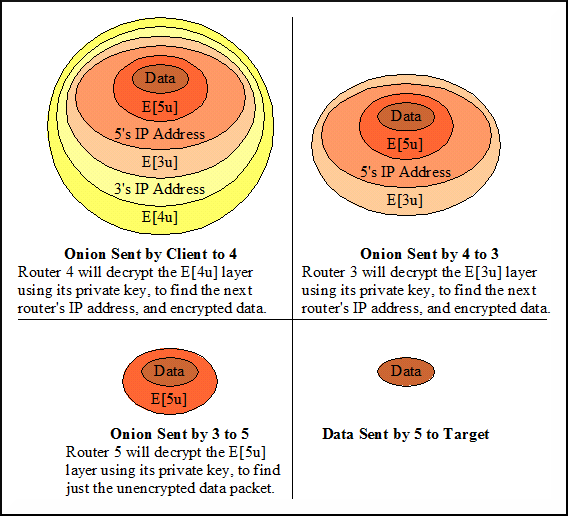
\includegraphics[width=0.5\textwidth]{anonion.png}
    \caption{Onion Routing \cite{cite4}}
    \label{fig:onion_image}
\end{figure}

\subsection{Advanced considerations}

Thera are many ways to attack \textit{Onion Routing} systems today: Denial of 
Service (DoS) attacks, Distributed Denial of Service (DDoS) attacks, passive 
tracking analysis, active tracking analysis.\cite{cite4}

Making \textit{Onion Routing} secure is a research area that grows from day to 
day with plenty of different ideas. \cite{cite4}

\subsubsection{Denial of Service (Dos) and Distributed DoS} 

As stated in the ``World Wide Web Security FAQ'': \textit{Denial of Service 
(DoS) is an attack designed to render a computer or network incapable of 
providing normal services. The most common DoS attacks will target the 
computer's network bandwidth or connectivity. Bandwidth attacks flood the 
network with such a high volume of traffic, that all available network 
resources are consumed and legitimate user requests can not get through. 
Connectivity attacks flood a computer with such a high volume of connection
requests, that all available operating system resources are consumed, and 
the computer can no longer process legitimate user requests.} \cite{cite5}

\textit{A Distributed Denial of Service (DDoS) attack uses many computers to 
launch a coordinated DoS attack against one or more targets.} \cite{cite5}

\subsubsection{Traffic Analysis}

The best way to protect from traffic analysis is to pay attention to the size 
of the onion (all onions should be the same size, regardless of the position
along the route) and make sure that timing information on circuits is well 
hidden. \cite{cite4}

\section{Tor}
\subsection{Overview}

Tor is a second generation and the most sophisticated implementation of the 
\textit{Onion Routing} protocol. The first important upgrade that Tor brings is
\textbf{perfect forward secrecy}: Tor now uses the \textit{``session'' key}
design, where the \textit{originator} negotiates with each node to derive a
shared secret --- the \textit{session key}. The \textit{session key} exchange
protocol which Tor uses is called Diffie-Hellman\cite{cite8} key exchange. The generated keys are only used for one
session, i.e. for the communication over one specific route. Public-key 
encryption is used only to establish the connection and secure the key exchange. \cite{cite4} \cite{cite6}

\textbf{Congestion control}: Tor has the ability to detect congestion and send
less data until the congestion goes down, while still maintaining anonymity. \cite{cite6}

\textbf{Directory servers}: A small set of very reliable servers act as 
\textit{directory servers}: they are able to control and monitor the chain 
nodes. Every active chain node has to register itself at the 
\textit{directory servers}, which then spread the information to all interested
clients. \cite{cite6}

\textbf{Leaky-pipe circuit topology}: \textit{Onion Routing} allows only the 
last node in the chain to be the \textit{exit node}. In Tor's implementation of 
the \textit{Onion Routing} protocol, this is changed allowing every node in the
chain to be the \textit{exit node}. \cite{cite4}

\textbf{End-to-end integrity checking}: Tor verifies data integrity at every
link of the chain in order to guarantee that no node in the chain can
change the data sent from the originator. \cite{cite6}

\subsection{Design}

\textit{Onion Routers} connect over a TLS-encrypted connection to other 
\textit{Onion Routers} in the network. Each user who uses Tor runs an 
\textit{onion proxy} to maintain the connections over the network, to 
communicate with the \textit{directory server} and to maintain the connections 
with the user's applications.\cite{cite6}

Each \textit{Onion Router} has an \textit{onion key} which is used to setup the
circuit and an \textit{identity key} which is used to register at the 
\textit{directory server} and to sign TLS certificates.  \cite{cite6}

The main units of communication in Tor are fixed-size data structures called 
\textit{cells}.\cite{cite6}

\subsection{Cells}

In Tor's design every \textit{cell} consists of a header and a payload and is
exactly 512 bytes long. The header of the \textit{cell} contains a circuit 
identification number (CircID), which is used to identify the individual logical
connection, and an instruction which tells the next node how to handle the 
payload. We can distinguish two types of \textit{cells},  \textit{control cells}
and \textit{relay cells}.\cite{cite6}

\textit{Control cells} consist of one of the following commands: 
\textit{padding}, \textit{create} and \textit{created} (create a new circuit), 
\textit{destroy} (destroy a circuit). \cite{cite6}

\textit{Relay cells} are special as they tell the receiving node to forward the
(encrypted) payload to the next node or a target server. The content of the 
\textit{relay cells} is encrypted using AES. The commands of the 
\textit{relay cells} are: \textit{relay begin} (open a stream), 
\textit{relay data}, \textit{relay end} (close a stream), 
\textit{relay connected} (successful  relay begin), \textit{relay teardown} 
(close a broken stream), \textit{relay extend} (extend the circuit), 
\textit{relay extended} (acknowledge of the  \textit{relay extend}),  
\textit{relay truncate} (terminate only part of the \textit{circuit}), 
\textit{relay truncated} (acknowledge of the  \textit{relay truncate}), 
\textit{relay sendme} (congestion control),  \textit{relay drop}.  \cite{cite6}

\begin{figure}
    \centering
    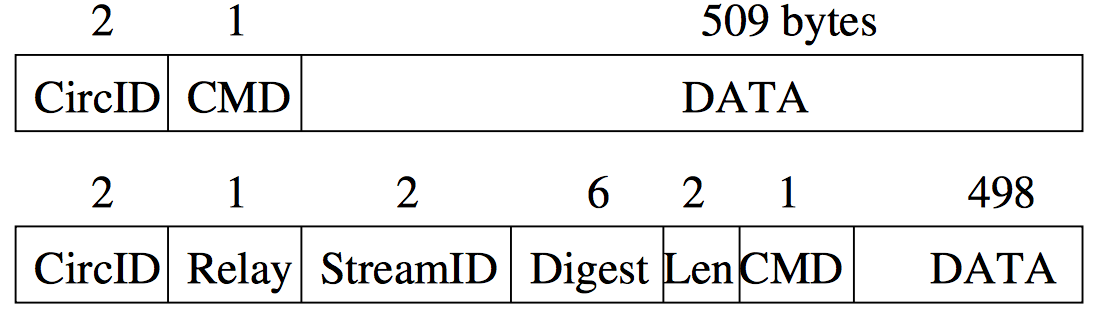
\includegraphics[width=0.5\textwidth]{cell.png}
    \caption{Cell \cite{cite6}}
    \label{fig:cell_image}
\end{figure}

\subsection{Construction of a circuit}

To create a \textit{circuit}, the originator's \textit{onion proxy} sends a 
\textit{create cell} (with a new CircID) to the first node, with a payload that
contains the first half of a Diffie-Hellman handshake. The first node responds 
with the \textit{created cell} containing the second half of this Diffie-Hellman
handshake as well as the hash of the generated shared secret. The onion proxy
can generate an identical shared secret using both halves of the Diffie-Hellman
handshake. At this point the \textit{circuit} between these two nodes is created
and they can send \textit{relay cells} to each other.  \cite{cite6}

\begin{figure*}
    \centering
    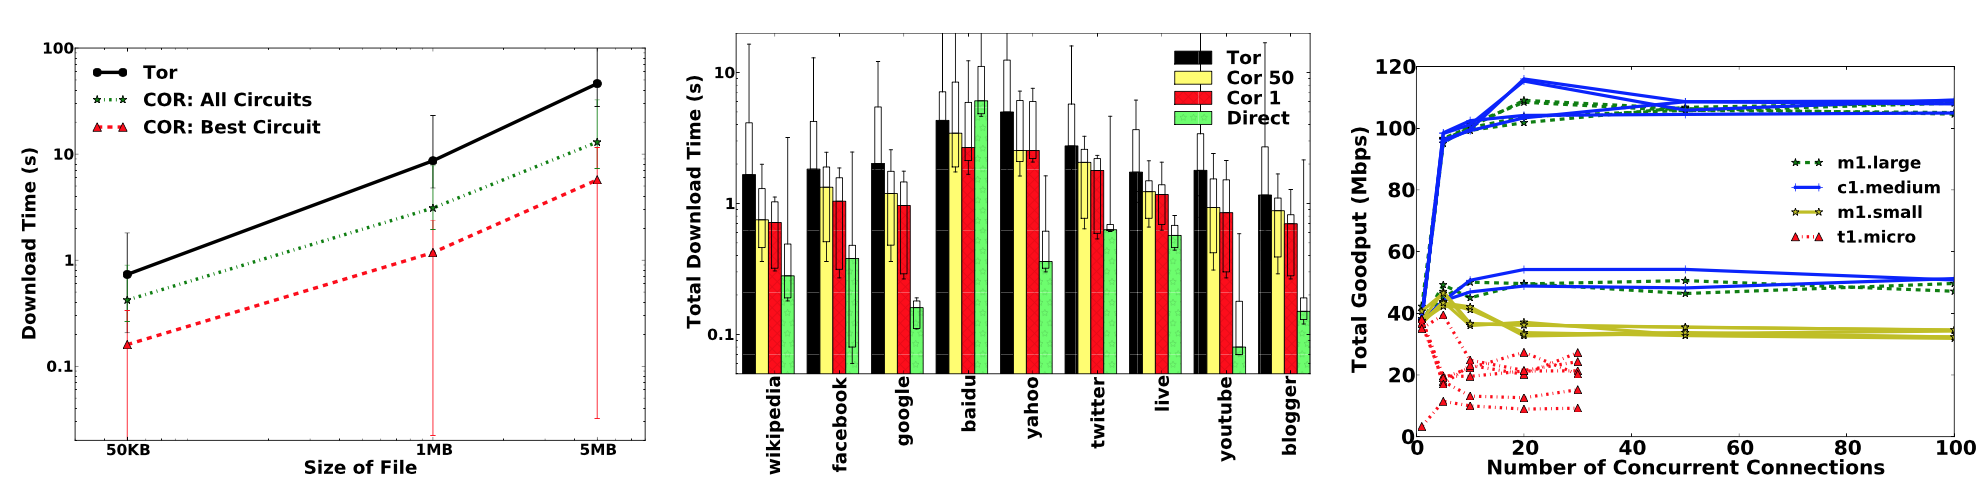
\includegraphics[width=1\textwidth]{evaluation.png}
    \caption{Evaluation \cite{cite2}}
    \label{fig:eval_image}
\end{figure*}

To extend the circuit to the next node, the originator's \textit{onion proxy} 
sends a \textit{relay extend cell} to the first node. The \textit{relay extend
cell's} encrypted payload contains the address of the second node and the first
half of a Diffie-Hellman handshake. The first node decrypts the payload and 
wraps the handshake data in a new \textit{create cell} (with new CircID) which
it passes to the second node. The second node responds to the first node with a
\textit{created cell}, along with its half of Diffie-Hellman and a hash of the 
shared secret. The first node encrypts and wraps this data in a 
\textit{relay extended cell} and passes it back to the originator. Now the 
\textit{circuit} is extended. \cite{cite6}

To extend the \textit{circuit} further, the above mentioned protocol is 
repeated by wrapping further \textit{relay} layers around the \textit{relay
extend cell}.

To completely tear down a \textit{circuit}, the originator sends a 
\textit{destroy cell} over the \textit{circuit}. Every node which receives such
a cell, closes the receiving \textit{circuit} and passes the 
\textit{destroy cell} forward. Because of the incremental nature of 
\textit{circuit} building, it is possible to tear down a circuit incrementally. 
The originator can send a \textit{relay truncate cell} to one node in the 
circuit. That node passes the \textit{cell} forward and replies with the 
\textit{relay truncated cell}. This way the originator is able to extend the 
circuit to different node. \cite{cite6}

\subsection{Opening and closing stream}

When the originator wants to open a new connection to the target, he sends a 
request to the \textit{onion proxy} to open a stream. By sending the 
\textit{relay begin cell} to the \textit{exit node}, the \textit{onion proxy} 
opens the stream. When the \textit{exit node} is connected to the target it
sends a \textit{relay connected cell}. Now the \textit{onion proxy} can send 
data over the circuit in a (sequence of) \textit{relay data cell(s)}. \cite{cite6}

We differentiate two types of cells for closing a stream. When the stream is 
closed normally, one node sends a \textit{relay end cell}, and the other side 
responds with its \textit{relay end cell}. For a stream that closes abnormally
(e.g., because of a connection timeout), the node next to the failed node sends
a \textit{relay teardown cell}. \cite{cite6}

\section{Performance evaluation: Tor and Cloud-based Onion Routing}

This evaluation considers two experiments for comparison: \cite{cite2}
\begin{itemize}
  \item downloading single files (TorPref)
  \item downloading entire web sites
\end{itemize}

\textbf{Individual Files Download:}

For performance evaluation when downloading single files, the Tor-supplied 
TorPref\footnote{https://metrics.torproject.org/tools.html} measurement tool was
used. The experiments used five \textit{cloud-based Onion Routing circuits} 
which were built over the US and EU datacenters, and five Tor circuits, randomly
built by Tor. Three files of size 50KB, 1MB and 50MB were downloaded, each 
download was repeated 100 times. The results are shown in the Figure 3 (left), 
and as you can see, the average \textit{cloud-based Onion Routing's} performance
is better then Tor's.\cite{cite2}

\textbf{Downloading Web pages:}

For this purpose 10 \textbf{entire} home pages were downloaded using Tor, 
\textit{cloud-based Onion Routing} and a direct Internet connection, and each 
home page was downloaded 10 times in a row. For the 
\textit{cloud-based Onion Routing} downloads, two use cases were tested, one 
with the \textit{cloud-based Onion Routing relay} under load (serving 50 
connections at the time) and serving just one connection at the time. In the 
Figure 3 (center) you can see that the \textit{cloud-based Onion Routing} is 
several times faster then Tor, although it is slower then direct access.\cite{cite2}

\textbf{Concurrent Users:}

Here the number of concurrent users that one node can maintain were evaluated. 
Also, for the purposes of this experiment, nodes with different performances
characteristics (nodes differ in CPU, memory and I/O resources) from Amazon EC2
were evaluated. It was shown that m1.large and c1.medium instances can maintain
more then 100 concurrent users, while the t.micro instance has problems with 
handling 10 users. The results are shown in Figure 3 (right) where you can see 
that the two largest instances achieved speed between 50 Mbps and 120 Mbps.\cite{cite2}

\section{Conclusion}
The goal of \textit{Onion Routing} is to protect anonymity by hiding the 
location and identity of its users. To fulfill its purpose 
\textit{Onion Routing} uses encryption to encrypt the original data 
and to create an onion. During its way towards the target the onion will be 
decrypted at each hop. When a router peels one encrypted layer of it only sees 
the address of the next router in the chain. Since no one can see the full path,
we can say that the communication is anonymous. \cite{cite4}

Because of elastic cloud infrastructure and powerful connectivity, 
\textit{cloud-based Onion Routing} introduces a new, more scalable level of 
implementation of \textit{Onion Routing} protocol. Also, 
\textit{cloud-based Onion Routing} brings additional level of protection against 
blocking, leaving censors with two options: allow the traffic or block all IP 
prefixes used by one cloud provider. Blocking all prefixes will cause a big 
damage: for example, Amazon EC2, hosted over a million instances with common IP
prefixes in 2010.\footnote{Recounting EC2 One Year Later: http://www.jackofallclouds.com/2010/12/recounting-ec2/}
Preliminary surveys demonstrates that \textit{cloud-based Onion Routing} can be
efficient, high performing and cost effective. \cite{cite2}.

\textit{Onion Routing} is an applied solution for real anonymity problems but 
yet still a big research area. \cite{cite7}

\bibliographystyle{plain}

\balancecolumns


\begin{thebibliography}{9}

\bibitem{cite1}
  Michael D. Reed, Paul F. Syverson, David M. Goldschlag, Naval Research Laboratory,
  \emph{Anonymous Connections and Onion Routing}, 1998.
  
  \bibitem{cite2}
  Nicholas Jones, Matvey Arye, Jacopo Cesaero, Michael J. Freedman,
  \emph{Hiding Amongst the Clouds: A Proposal for Cloud-based Onion Routing}, Princeton University, 1998.
  
  \bibitem{cite3}
  Michael D. Reed, Paul F. Syverson, David M. Goldschlag, 
  \emph{Onion Routing for Anonymus and Private Internet Connection}, 1998.
  
    \bibitem{cite4}
  Marc O'Morian, Vladislav Titov, Wendy Verbuggen, 
  \emph{Onion Routing for Anonymus Communication},
  http://ntrg.cs.tcd.ie/undergrad/4ba2.05/group10/
  
      \bibitem{cite5}
  Lincoln Stein, John Stewart, 
  \emph{The World Wide Web Security FAQ: Securing against Denial of Service attacks},
  http://www.w3.org/Security/Faq/wwwsf6.html
  
    \bibitem{cite6}
  Roger Dingledine, Nick Mathewson, Paul Syverson, 
  \emph{Tor: The Second-Generation Onion Router}.
  
  \bibitem{cite7}
Paul F. Syverson,  Naval Research Laboratory,
  \emph{A Peel of Onion}.
  
  \bibitem{cite8}
  W. Diffie, M.E. Hellman,
  \emph{New directions in cryptography, IEEE Transactions on Information Theory}, 644-654, 1976.

\end{thebibliography}

\end{document}
